\begin{frame}{Gewinner und Übergabe}
\begin{columns}[T,onlytextwidth]
\begin{column}{0.48\textwidth}
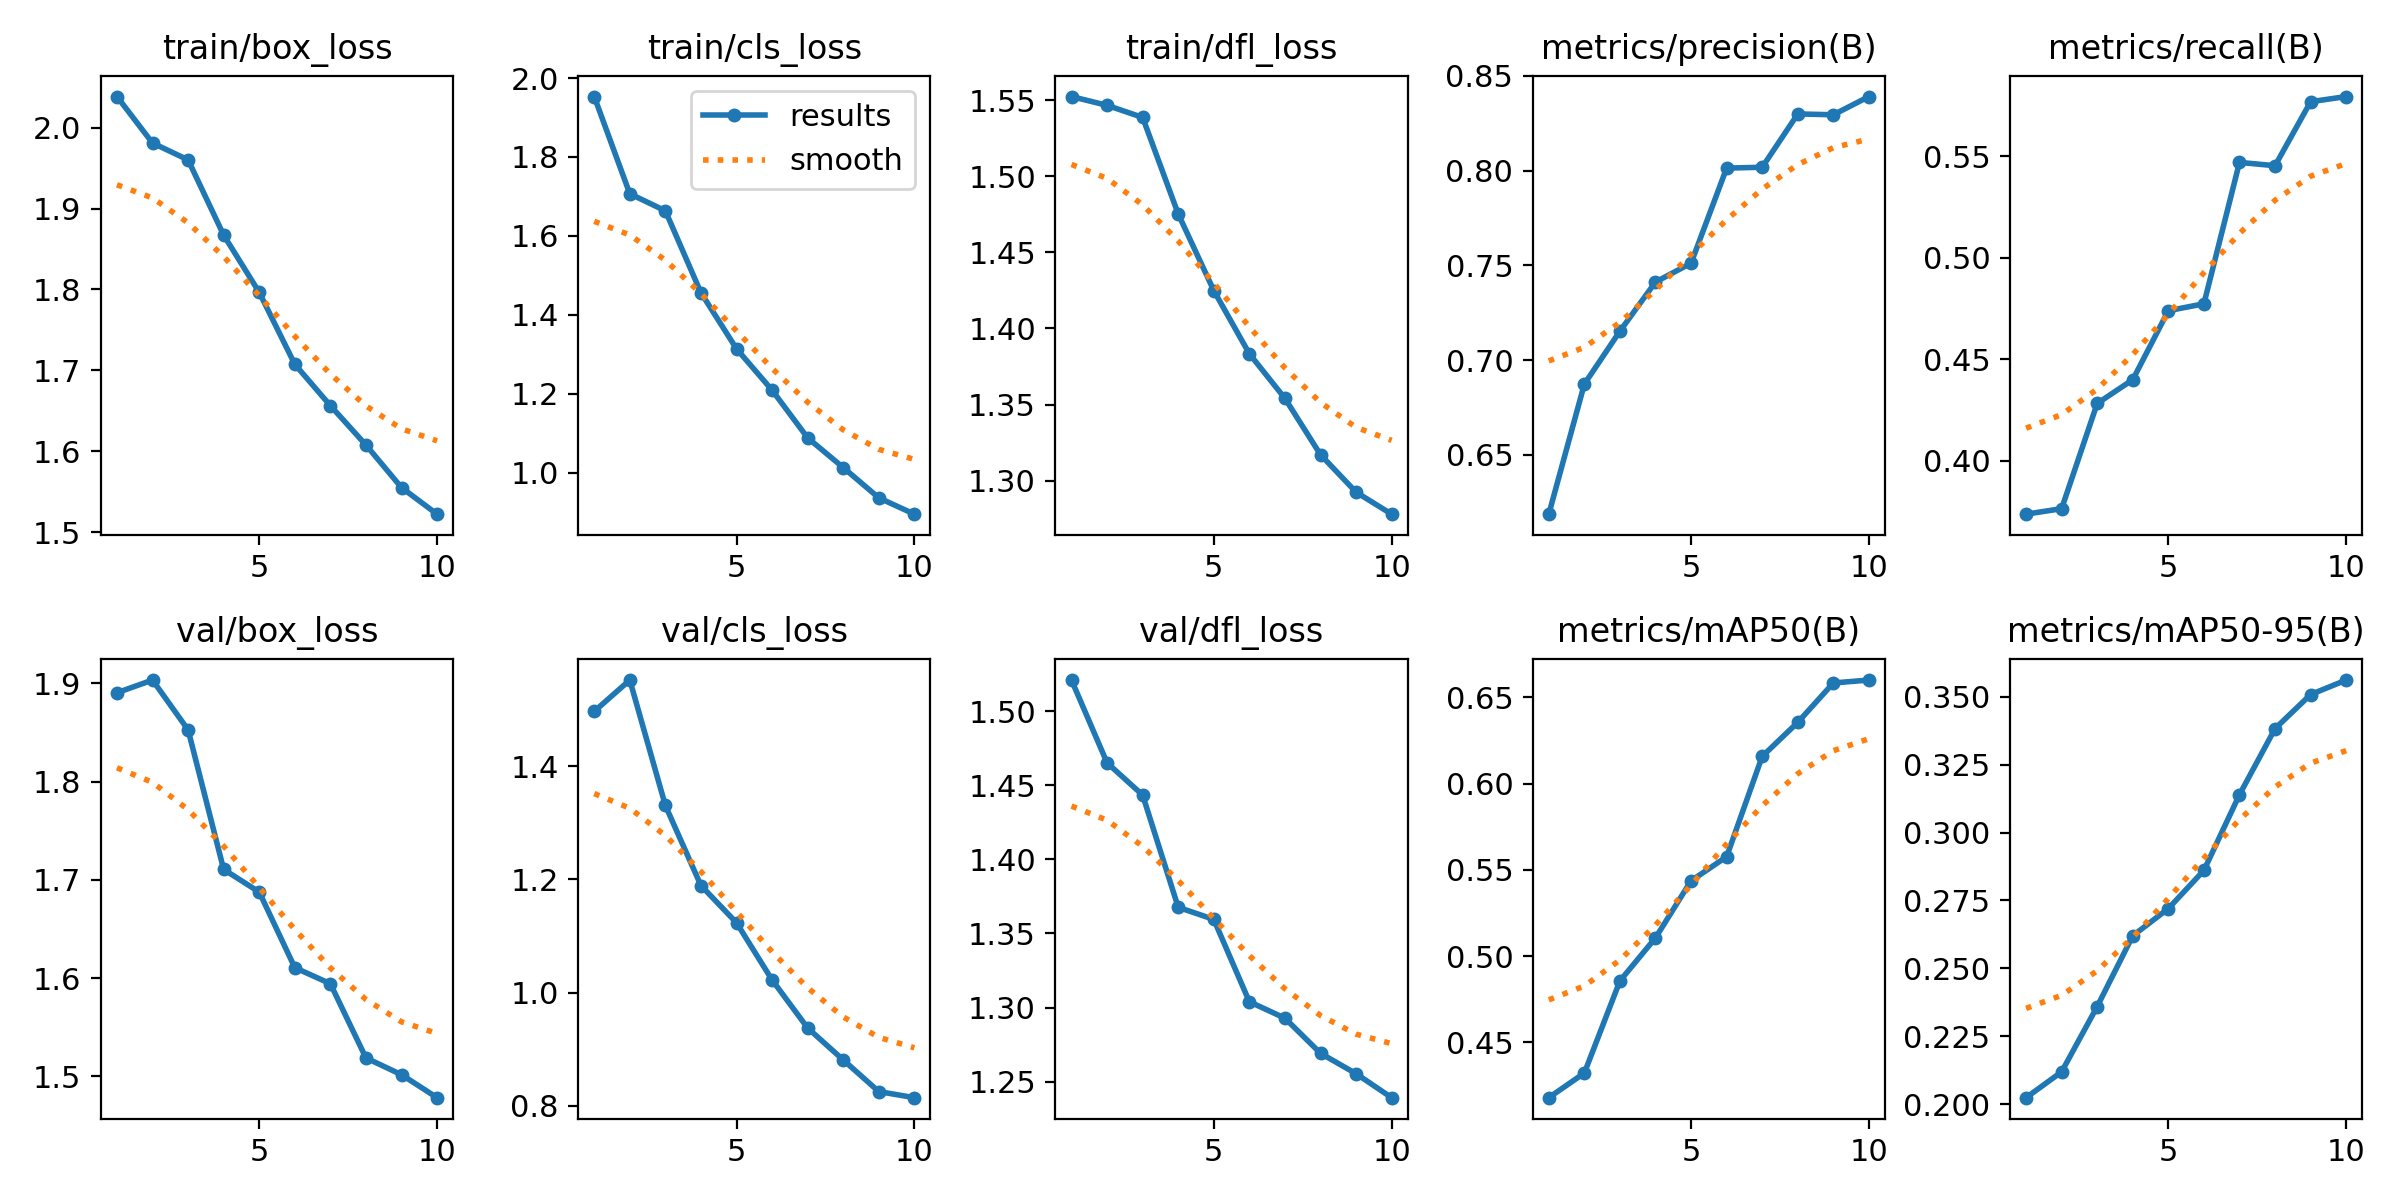
\includegraphics[width=\textwidth,height=0.26\textheight,keepaspectratio]{imglib/face_model_lab/yolo_results.png}
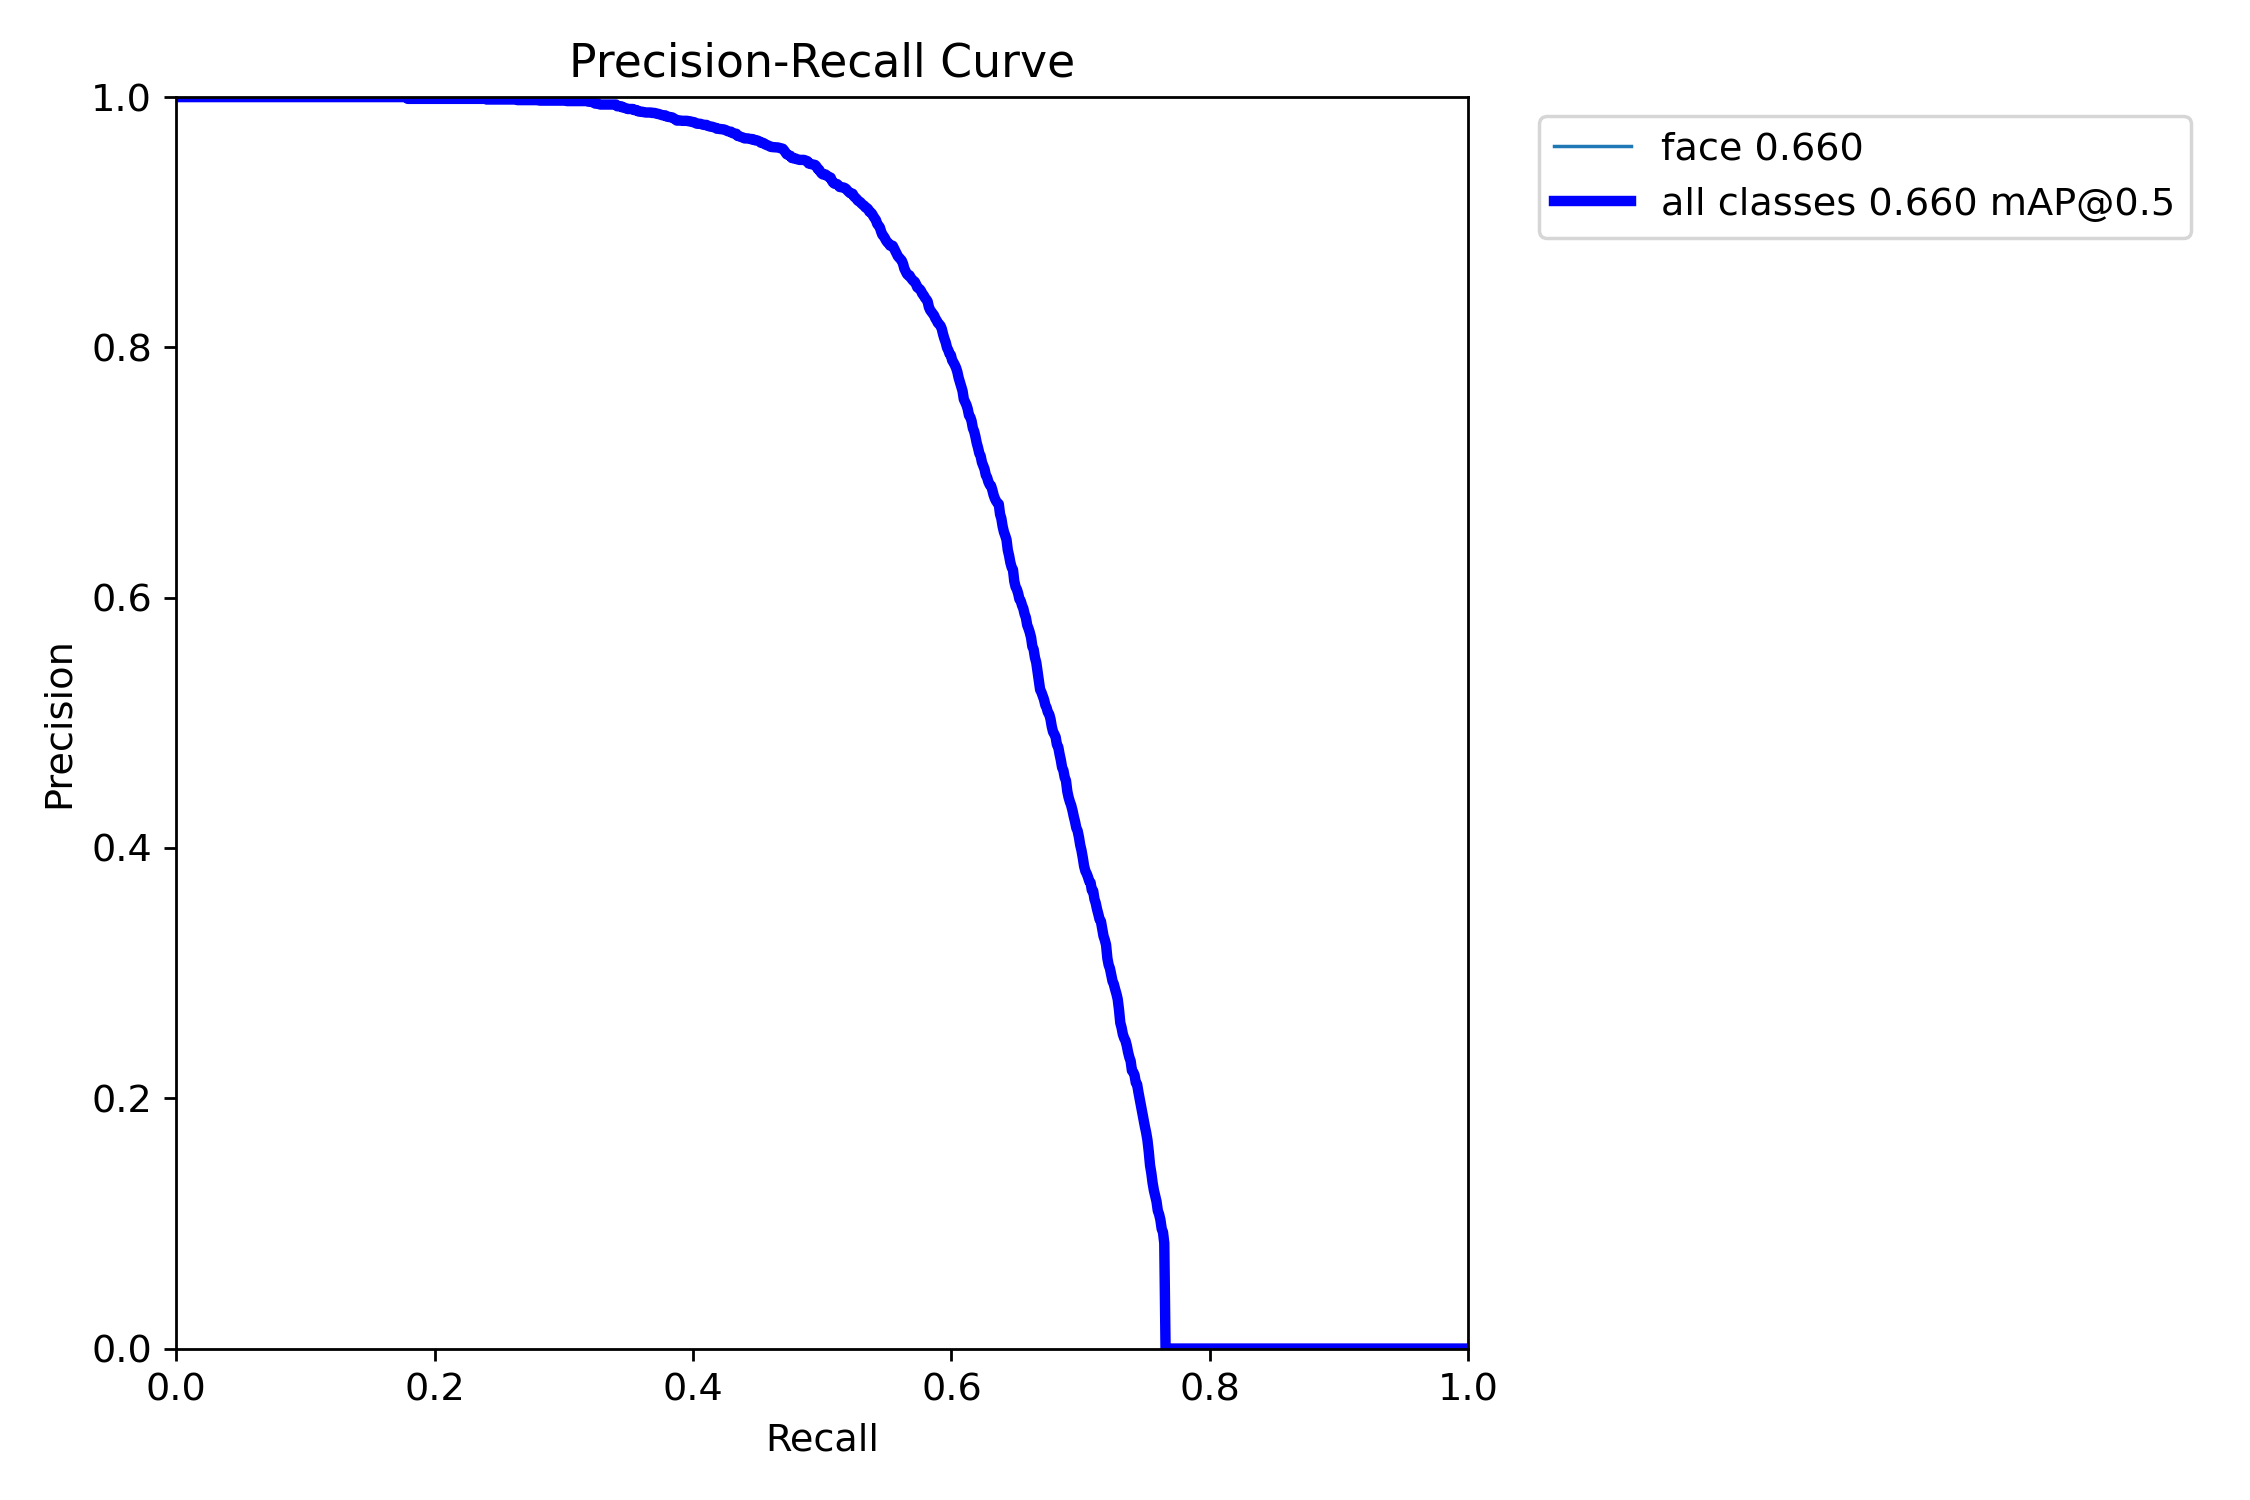
\includegraphics[width=\textwidth,height=0.18\textheight,keepaspectratio]{imglib/face_model_lab/yolo_box_pr_curve.png}
\end{column}
\begin{column}{0.48\textwidth}
\scriptsize
\begin{itemize}
    \item FCOS und YOLOv8m sind die Gewinner der Vorauswahl: Qualität gegen operative Einfachheit.
    \item Faster R-CNN wird als starker Red20-Kandidat in den großen Red6/10-Vergleich nachgezogen.
    \item Die finale Entscheidung betrachtet Recall, Validierungsmetriken, Latenz, Modellgröße und Video-Pipeline.
\end{itemize}
\end{column}
\end{columns}
\vspace{0.2em}
\begin{mynote}[Übergabe]
\scriptsize
Video-Übergang: erst ungeblurrtes Original, dann dieselbe Szene mit YOLO-Blur und Qualitätsbewertung. So werden Recall, Box-Grösse und Blur-Qualität sichtbar.
\end{mynote}
\end{frame}
